\documentclass[abstract=on,12pt]{scrreprt}

% Set packages to be used
\usepackage[rightcaption]{sidecap}	% Allows for figures with captions on the side, rather than the top/bottom
\usepackage[hidelinks]{hyperref}	% Adds support for hyperlinks
\usepackage[british]{babel}			% Set the language to UK English
\usepackage[a4paper]{geometry}		% Set the paper type
\usepackage[T1]{fontenc}			% Change the encoding to allow for more character types
\usepackage{booktabs}				% More professional looking table layouts
\usepackage{csquotes}				% Easy quotation
\usepackage{enumitem}				% Nicer itemizations
\usepackage{etoolbox}				% Lets you do fancy stuff with section types
\usepackage{fancyhdr}				% Fancy Headers
\usepackage{graphicx} 				% For loading graphic files
\usepackage{multicol}				% Used to set column counts
\usepackage{pdfpages}				% Used to include external PDFs in the document
\usepackage{ragged2e}				% for '\RaggedRight' macro (allows hyphenation)
\usepackage{setspace}				% Sets the spacing between lines
\usepackage{tabularx}				% for 'tabularx' environment and 'X' column type
\usepackage{titlesec}				% Allows custom formatting for sections
\usepackage{apalike}				% Format references in APA styling
\usepackage{gensymb}				% Allow inclusion of special characters, such as degrees
\usepackage{lmodern} 				% Type1-font for non-english texts and characters
\usepackage{wrapfig}				% Allows wrapping figures in text blocks

% Set document specific info
\title{Is Immersion Possible in Non-Euclidean Virtual Environments?}
\subtitle{CHP2524 - Individual Project Report}
\author{Nathan Boxhall-Burnett}
\setlength{\columnsep}{1cm}			% Set the spacing between columns
\onehalfspacing						% Set the spacing between the lines of text
\graphicspath{Images/}				% Set the default path to use for images

% Set the page number and running title as header
\pagestyle{fancy}
\fancyhf{}
\fancyheadoffset{0cm}
\renewcommand{\headrulewidth}{0pt}
\renewcommand{\footrulewidth}{0pt}
\fancyhead[R]{\thepage}
\fancyhead[L]{Is Immersion Possible in Non-Euclidean Virtual Environments?}
\fancypagestyle{plain}{%
	\fancyhf{}%
	\fancyhead[R]{\thepage}%
	\fancyhead[L]{Is Immersion Possible in Non-Euclidean Virtual Environments?}
}

% Set formatting for chapter titles
\titleformat{\chapter}[hang]{\huge\bfseries}{\thechapter}{1em}{\huge}

% Set formatting for section titles
\titleformat{\section}[hang]{\large\bfseries}{\thesection}{1em}{\large}

% Set formatting for section titles
\titleformat{\subsection}[hang]{\normalsize\bfseries}{\thesubsection}{1em}{\normalsize}

% Add the abstract to the table of contents
\patchcmd{\abstract}{\titlepage}{\titlepage
	\addcontentsline{toc}{chapter}{Abstract}}{}{}

% Begin the document
\begin{document}

	% Title Page
	\maketitle

	% Set the inital pages to use roman numerals for numbering
	\pagenumbering{roman}

	% Table of contents
	\tableofcontents

	% Abstract
	\begin{abstract}
		\thispagestyle{plain}
		%expression of general problem/area

		%specific problem/objective attempted

		%what you have achieved

		%lessons learned

		%% DO NOT START BY SAYING WHAT YOU HAVE DONE 
		%% DO NOT INCLUDE JARGON / DETAILS 
		% Eg bad start “I have implemented a C\# database running on Linux v4.5.2 … “
		% Eg bad start “ I have created a web application” – start with overview and problem area first.
		%% MAKE IT UNDERSTANDABLE TO ALL ! 


		With Virtual Reality (VR) development and availability increasing as rapidly as it has in recent years, experiences that are capable from Virtual Environments (VE) that are not limited to the restrictions of the real world, and the effectiveness they have in a users perception and sense of immersion, need to be considered.
		Studies surrounding a users interaction in VR environments that have taken place previously tend to focus on how reliably the user can interact with an environment mimicking the real world.
		This study attempts to fill the gap in existing research by examining the effects non-Euclidean geometry has on a users sense of immersion in VR.
		% TODO Talk about data gathering
		% TODO Talk about results

		%This review explores the existing literature that covers the various requirements for creating a VE that consumers would perceive as \enquote{realistic} in VR.
		%As well as this, it also covers how these requirements have been, and can be, adapted to work inside of a world which does not follow the restrictions of real world geometry, such as in non-Euclidean or Escheresque space.
		%Gaps in the current literature are outlined, alongside prospective areas for future research.
	\end{abstract}

	% Set formatting for section titles
	\titleformat{\chapter}[hang]{\large\bfseries}{\thechapter}{1em}{\large}

	% Remove section numbering for the acknowledgements
	\setcounter{secnumdepth}{-2}

	% Document Acknowledgements
	\chapter{Acknowledgements}
		I would like to thank my supervisor Hugh Osborne, and examiner Duke Gledhill, for their invaluable feedback and suggestions throughout.
		I would also like to thank all the participants who took the time to take part in the product experiments.

	% Set formatting for chapter titles
	\titleformat{\chapter}[hang]{\huge\bfseries}{\thechapter}{1em}{\huge}

	% Reset the page count, reset the numbering style to arabic, and add section numbering again
	\newpage
	\renewcommand\thepage{\arabic{page}}
	\pagenumbering{arabic}
	\setcounter{secnumdepth}{3}

	% Introduction
	\chapter{Introduction}
\label{intro}
\begin{multicols*}{2}

	%explains  context, the problem/area, the clients / users / target audience. Also it should give a summary of what you have achieved and what your deliverable is.

	%% HINT: Start by introducing the reader to the area, then explain what the specific problem/area you have tackled is and then what you have achieved.
	%% MAKE IT CLEAR WHAT YOU HAVE DONE/ACHIEVED
	%% COMPLETE YOUR INTRODUCTION AFTER YOU HAVE FINISHED THE REST OF THE PROJECT REPORT!


	%Here I will be introducing the project and the various sections of the report document in detail, making sure to cover the terms and concepts that will be discussed to ensure the reader has full understanding of the report contents.

\end{multicols*}

	% Literature Review
	\chapter{Literature Review}

	% Intro Page
	\section{Introduction}
\label{lr:intro}
%	Here I will be introducing and outlining the concepts that will be covered in the following sections.
	
\begin{multicols*}{2}
	Virtual Reality (VR) is fast becoming a mainstream platform for video games, with high quality devices allowing the feeling of 'presence' in a game world being released for computers, game consoles, and mobile devices alike, creating a vast user base for potential products.
	
	As well as this, the popularity of video games which utilise non-standard or real-world geometric principles are also increasing, with the popularity of titles such as Antichamber \cite{Antichamber2013} and Portal 2 \cite{Portal22011} engaging consumers with their non-conformity to the physics and geometry of average game worlds.
	
	This review is split up into three chapters, each one covering a specific area of existing literature relevant to it:
	\begin{enumerate}
		\item \nameref{lr:vr}, which will cover various elements creating a sense of presence in a Virtual Environment (VE) using VR requires, such as user perception and affordances
		\item \nameref{lr:ne}, which will cover existing applications of non-standard geometry in video game systems
		\item \nameref{lr:cross}, which will cover how the requirements from the previous chapters are to be utilised together to form a working system, as well as the tools which are best suited for constructing such a system
	\end{enumerate}
	
\end{multicols*}


	% Requirements for Presence in Virtual Reality chapter
	\section{Presence in Virtual Reality}
\label{lr:vr}

\begin{multicols*}{2}
	
	\subsection{Introduction}
	\label{lr:vr:intro}
	%		This section will introduce the key concepts that will be discussed in the following subsections.
		Presence is the term used in VR systems to describe a user's sense of existing inside a VE. Because of this, it can be seen as one of, if not the most important feature of the design for a VR system.

		There are a few main features which are key to achieving a sense of presence in a VE. One example would be the general perception of the user for things such as depth perception, the ability for a person to calculate the distance of a point from themselves, and sensorimotor adaptation, which is the calibration of a user's senses to fit their environment.
		As well as this, there are specified areas such as affordance detection, the ability for a person to calculate interaction with an object or environment, which helps assist a user with navigation and interaction in a VE.
		The following sections will review existing literature on the aforementioned features.
	
	\subsection{Affordances in VR}
	\label{lr:vr:affordances}
	%		Here I will introduce the concept of, and cover research into affordances in Virtual Reality.
		%Perceiving affordances in virtual reality: influence of person and environmental properties in perception of standing on virtual grounds
		Affordance is especially important to get right in VR, particularly in a video game environment, due to the world a user is in is designed to be interacted with.
		Unlike what common sense would dictate, research on affordance in the real world may not be as applicable for when designing interactions in a virtual world as expected.
		A study \cite{Regia-Corte2012} focusing on a person's perception for whether or not they could stand upright on an object at various angles in a virtual world found that, contrary to expected results, users would tend to be more cautious when judging their ability in a virtual environment (critical angle 21.98\degree) compared to an equivalent object in the real world (critical angle 30\degree), even with a lack of apparent risk.

		This study covered the various requirements for the experiments well, however there were a few areas in which it could still be expanded upon.
		These areas include comparing results from using a variety of VR systems to judge responses based on hardware response times, display resolutions, and refresh rates, as well as increases and decreases in model and texture quality (not just the texture itself as they did) for judging the surfaces of the objects.

		% Designing presence for real locomotion in immersive virtual environments: an affordance-based experiential approach
		Another way in which affordance directly affects a user's sense of presence in VR is the simulation of real locomotion for the user.
		In a study \cite{Turchet2015} covering the ways in which a user's movement is recorded and displayed in a VE (including, but not limited to, individual foot tracking, arm, leg, and head tracking, movement speed tracking, etc.), results found that while an increase in the coverage of the input also increased the sense of presence for the user, it was more important to focus the areas based on their relevance to the scenario at hand.
		As well as this, the study found that while the input tracking itself was important, to attain a greater sense of presence it was also required for the physical representation of the user to match their real physical selves as much as possible, such as gender, height, and weight.

		This study, while extremely thorough in its coverage of the various possible elements required to generate a sense of presence, could have recorded and displayed its results in a more usable manner than it did.
		Due to the way the experiments were conducted, the results do not indicate any sense of importance for each individual step in its contribution to the feeling of presence in the user.
		Because of this, further research could be undertaken to create a weighted system designed around the experiments conducted, signifying its importance for specific VR systems, creating a more convenient set of data for future use.

	\subsection{Perception in Virtual Environments}
	\label{lr:vr:perception}
		This section will cover existing research into how people perceive environments in Virtual Reality.
		% Using virtual reality to augment perception, enhance sensorimotor adaptation, and change our minds.
		Perception is a key feature to get right in VR, as incorrect calibration for features such as head tracking and input response can have both unintended, and undesired side-effects. In studies \cite{Wright2006}  \cite{Wright2009} \cite{Wright2011} \cite{Wright2013} \cite{Wright2014} around the effects of perception augmentation and sensorimotor adaptations, results showed that tests around sensorimotor processes that made use of Virtual Reality systems could have both intended and unintended effects on the participants central nervous system. 
		(NOTE) This paragraph needs expanding upon


		% Immersive Virtual Environment Technology to Supplement Environmental Perception, Preference and Behavior Research: A Review with Applications

		(PLACEHOLDER) Discuss \cite{smith2015} - Immersive virtual environment technology to supplement environmental perception, preference, and behaviour research

	\subsection{Conclusion}
	\label{lr:vr:conclusion}
		Here I will summarise the concepts and sources discussed in the previous sections, how reliable they may be, and how the concepts could apply to my project.
		Due to recent relevant technology being both of a high quality, and low enough cost to warrant consumer interest, as well as its applications in not just Video Games, but in Medicine, Psychology, and Education, Virtual Reality is a very highly researched area.

		Studies have been conducted to cover an extremely wide range of applications and effects for VR, and because of this, there is a very solid foundation of work which can be both applied for practical uses, as well as a platform to build upon for future research.

		This is especially true in the two main focus points for the literature covered in this review, and will be beneficial for reference during the creation of the proposed system.

\end{multicols*}


	% Non-Standard Geometry chapter
	\section{Non-Standard Geometry in Game Engines}
\label{lr:ne}

\begin{multicols*}{2}
	\subsection{Introduction}
	\label{lr:ne:intro}
%		In this section I will introduce the concept of non-standard geometry, e.g. non-Euclidean, and review existing literature regarding its use in video game engines.
	
	\subsection{Existing Examples}
	\label{lr:ne:existing}
%		Here I will cover literature around non-Euclidean geometry, as well as existing examples of such geometry in virtual environments.
		(PLACEHOLDER) The following sources will be discussed in this section:
		\begin{itemize}
			\item \cite{Maric2014} - Formalizing complex plane geometry
			\item \cite{Turner2009} - Mathematics and the Imagination
			\item \cite{Lindley2005} - Game space design foundations for trans-reality games
		\end{itemize}
		
	\subsection{Conclusion}
	\label{lr:ne:conclusion}
		This section will be used to sum up the sources discussed above, how relevant and reliable they are as sources, and how they relate to my project.
		
\end{multicols*}


	% Application of Virtual Reality in a Non-Euclidean world Chapter
	\section{Application of VR in Non-Euclidean worlds}
\label{lr:cross}

\begin{multicols*}{2}
	\subsection{Introduction}
	\label{lr:cross:intro}
%		In this section I will introduce the concepts to be covered in this section, namely how one can apply the key concepts for perception and presence in VR to a game world using non-standard geometry.
	
	\subsection{Application}
	\label{lr:cross:application}
%		Here I will be covering any existing research which relates to the combination of VR and non-Euclidean geometry.
		(PLACEHOLDER) The following sources will be discussed in this section:
		\begin{itemize}
			\item \cite{Cruz-Neira1993} - Surround-screen projection-based virtual reality
			\item As referenced in \ref{lr:vr:perception}, \cite{Wright2014} - Using virtual reality to augment perception, enhance sensorimotor adaptation, and change our minds - Discuss how it could also relate to sensorimotor adaptations allowing a user to get accustomed to existing i\textsl{}n a non-Euclidean world.
		\end{itemize}
	
	\subsection{Tools \& Techniques}
	\label{lr:cross:tools}
%		This section will cover tools which are applicable for the creation of VR/Non-Euclidean virtual environments.
		(PLACEHOLDER) In this section I will be covering the various tools I could use to create the proposed system, these tools and techniques will include:
		\begin{itemize}
			\item Software 
			\begin{itemize}
				\item Custom engine
				\begin{itemize}
					\item Oculus SDK 0.8
					\item NVIDIA Gameworks VR
					\item AMD LiquidVR
					\item DirectX 11.2 / 12
					\item OpenGL 4.5
				\end{itemize}
				\item Modify existing engine
				\begin{itemize}
					\item Unity 5
					\item Unreal 4
				\end{itemize}
			\end{itemize}
			\item Hardware
			\begin{itemize}
				\item Head-Mounted Display
				\begin{itemize}
					\item Oculus Rift DK2
					\item HTC Vive
				\end{itemize}
				\item Input
				\begin{itemize}
					\item Keyboard/Mouse
					\item Game controller (PS4, XBox One, etc.)
					\item Web-cam/Kinect
				\end{itemize}
			\end{itemize}
			\item Project Management
			\begin{itemize}
				\item Time Planning
				\begin{itemize}
					\item Agile
					\item Waterfall
				\end{itemize}
				\item Source Control
				\begin{itemize}
					\item Git
					\item SVN
				\end{itemize}
			\end{itemize}
		\end{itemize}
		Resources for reference:
		\cite{Bruce2012} - Custom engine v modify an existing one - debate. Compares the pros and cons of both modifying an existing engine and creating a custom solution. ('Leaky Abstractions' with an existing engine, balance engine efficiency and actual system development with a custom engine, etc.).
		
	\subsection{Conclusion}
	\label{lr:cross:conclusion}
%		This section will sum up the points discussed in the above subsections.
		(PLACEHOLDER) Sum up the points discussed in the above sections. Example: current implementations of non-euclidean geometry in released games have always directly used, or modified an existing generic game engine to create the VE, and are therefore not optimised to be used in a non-euclidean world.
	
\end{multicols*}


	% Conclusion
	\section{Conclusion}
\label{lr:conclusion}
%	Here I will be summarising the state of the existing literature from the previous sections, and outlining any gaps in the research.

\begin{multicols*}{2}
	In Virtual Reality, non-standard geometry is definitely an area with potential to engage, and possibly spark an interest within a user about the capabilities and uses of such concepts.
	
	This paper has given an overview into the various components required for the creation of an environment suitable for use in VR, how non-standard geometrical worlds can be created for use in a VE, and how the areas both require adaptation in order to work together.
	
	In terms of Virtual Reality, existing literature is very thorough in its coverage of the possibilities and effects of its use both within and outside of video game environments. Although there is definitely still room for further research into the more niche areas of study, there is a solid foundation for use as a reference for development in the field.
	
	For non-Euclidean geometry, however, there is a distinct lack of academic research into its use within virtual environments, with most studies focusing instead on the theoretical applications for it. Reports around the use of non-standard geometry in video games does exist, however due to the non-scholarly nature of the sources, which are mainly video game journalist articles or developer interviews, they cannot be completely trusted for academic purposes.
	
	Due to combination of the findings surrounding these areas, future research into the use of non-Euclidean geometry within a VR system is very open to exploration, and as such, research would be beneficial as a possible basis for further study, perhaps even encouraging it.
\end{multicols*}


	% Maybe other background stuff too, who knows

	% Models/Product Design stuff
	\chapter[Product]{Design and Implementation}
\label{design}

	\section{Introduction}
	\label{design:intro}

		Due to the room for research available in this area, it made sense to focus this study on a relatively broad area of the subject to be used as a foundation, rather than to specialise on a particular niche.
		% REWORD THIS?
		Because of this, the main focus for this study is the effects that Non-Euclidean geometry has on a user's sense of Immersion, and to find any changes in a user's comfort navigating in a virtual environment.

		This chapter covers the development process that was undertaken for the creation of the product used for the experiments.

	%\section{Development Process}
	%\label{design:dev}
	% TODO: This, if we get time

		% this section will cover the development process of the product itself

		% Talk about development methodologies considered for use with the project, and how they were adapted for use for a single person.
			% Use of Git and stuff like that

		% Talk about how you decide to use an existing engine you knew well (save time reinventing the wheel for things like lighting, camera stuff, etc)
		% Also you wanted to limit the amount of outside variables as possible, so an existing engine helped with that


	\section[Implementation]{Product Implementation}
	\label{design:model}

		To achieve the effect that a player is inside a non-Euclidean environment, a total of three primary pieces of functionality needed to be implemented:
		\begin{enumerate}
			\item A way to position a camera in a way to get the perspective of an area which would be seen by the player of the area which would give the impression of non-Euclidean space
			\item A way to render the new perspective to be seen by the player, but only in desired areas
			\item A way to transport the player between their current position and the new perspective without them realising they have gone anywhere other than they expected.
		\end{enumerate}

		To calculate the relative position for a camera to render a new perspective for the player, two pieces of information needed to be known: the plane where the player would be viewing the perspective from (hereby referenced as \enquote{from plane}), and a plane in the new area that the player would be viewing the perspective of (hereby referenced as \enquote{to plane}). Both planes can be seen referenced by the two \enquote{View Area} lines in \autoref{design:fig:maths}.
		With the two relative points known, the next step is to work out the positioning and rotation that the camera will need to use for the new area.
		The position of the camera could be worked out by calculating the distance vector between the player and the \enquote{from plane}, represented by \enquote{A} (Z axis) and \enquote{B} (X Axis) on \autoref{design:fig:maths}, with an unseen \enquote{C} which would represent the distance in the Y axis.
		The position offset then needs to be reoriented by the difference in rotation between the \enquote{from plane} and \enquote{to plane}, before finally being translated relative to the position of the \enquote{to plane}.
		This calculation can be seen in lines 90 or 93 in \autoref{appendix:code:camera}.

		\begin{figure}[h]
			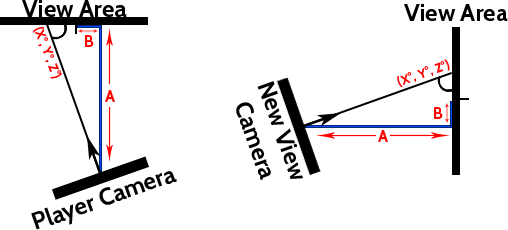
\includegraphics[width=0.8\textwidth]{Images/Position}
			\centering
			\caption{Top-down 2D representation of the calculations for the position and rotation of cameras.
				See \autoref{appendix:code:camera} for the implementation}
			\label{design:fig:maths}
		\end{figure}

		The next step was to calculate the rotation to use for the camera.
		In order to find out the rotation that is needed for the camera, two calculations needed to be made.
		The first is one which was done before, which is the difference in rotation between the \enquote{from plane} and the \enquote{to plane}.
		The second is the difference in rotation between the player camera, and the normal of the \enquote{from plane} (Represented by \enquote{(X\degree, Y\degree, Z\degree)} in \autoref{design:fig:maths}).
		With these two rotations known, the final rotation of the perspective camera can be calculated.
		This calculation can be seen in lines 91 or 94 in \autoref{appendix:code:camera}.
		% TODO: Talk about the problems with some portals needing their positions and rotations inverted!

		One of the more challenging aspects for achieving the non-Euclidean effect in the scene was getting the new perspective camera to render appropriately in the scene itself.
		The usual approach for rendering different views in Unity is to use their provided \enquote{Render Textures}, which allow you to render a camera to a texture, and use that as the texture of an object in the game world.
		Although that method works well for regular games outside of VR for things like mirrors, it was not a valid solution for use in VR where the user can perceive depth in the virtual environment, due to the texture being rendered on a flat mesh.

		To get around this issue, a custom shader was made (\autoref{appendix:code:shader}) which could be applied to an object which was acting as the area for where a user should see the new perspective.
		This shader had three main features: it would write the position of the object to the Z buffer for the render queue to ensure nothing behind it would be rendered, it would write no data to the RGBA (colour) channels to ensure nothing would be visibly rendered in that position from the players perspective, and finally it would always be the last thing to be rendered in the scene (Other than UI elements) to ensure the area would always be clear.

		\begin{figure}[h]
			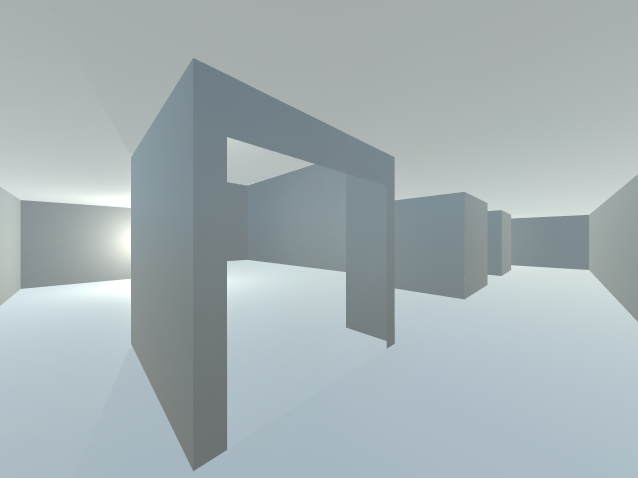
\includegraphics[width=0.66\textwidth]{Images/NE_View}
			\centering
			\caption{Example of view of the final effect inside the Non-Euclidean scene, displaying an area which appears larger than the container surrounding it}
			\label{design:fig:game}
		\end{figure}

		With objects placed in the scene with the shader, it would allow the view from the new perspective cameras, which had their own render queues so the effect would not overwrite them, to be drawn in place of those objects.
		When coupled with the correct positioning and rotations of the perspective camera, it gave the impression that the other perspective was directly in those areas, in full stereoscopic 3D (As seen in \autoref{design:fig:game}).
		% TODO: properly proof read this section

		With the illusion working properly visibly, the final step was to allow the user to navigate between the areas in a way that gives no indication to the user that they have been transported.
		The calculations for the actual positioning of the player once being transported were similar to that of the perspective camera positioning, where it would calculate a position for the player, and a rotation for the camera, relative to the \enquote{to plane} and \enquote{from plane} (\autoref{appendix:code:player}).
		The next calculation which needed to be done for the player positioning was to know when to transport the player.
		To do this, a collision area was added to the \enquote{plane from} and \enquote{plane to} objects.
		In the collision areas, instead of stopping the player from moving within them, they would be used to detect if the player has moved greater than half way through the area, and if so, they would be transported to the equivalent area in the connected plane (\autoref{appendix:code:player} line 142).
		From here, the only additional calculation that needed to be made was to adjust the vector containing the players movement momentum, and adjust it to be relative to the rotation offset between the two planes.

		As a way of assisting with the modelling of the scenes themselves, lines were drawn inside the scene views of the Unity editor which would symbolise the various aspects of the connected points (\autoref{design:fig:scene}).
		In the figure, red lines indicate the locations of the \enquote{to plane} and \enquote{from plane} for the connections, green lines indicate the normals of the planes, and yellow lines indicate planes which are visible to the player at any given time.
		Only planes which are currently visible by the player have their respective perspective cameras positioned and rendered.

		\begin{figure}[H]
			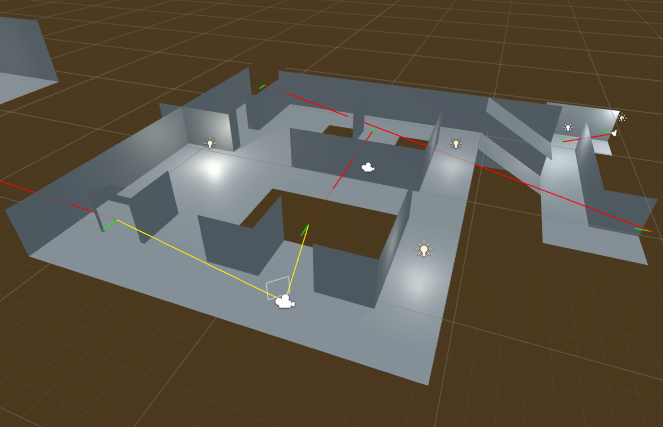
\includegraphics[width=0.85\textwidth]{Images/Lines_Everywhere2}
			\centering
			\caption{Example view of a scene in the Unity editor.}
				%Red lines are connections between points,
				%yellow lines are connections visible to the player,
				%and green lines are the direction the connectors are facing}
			\label{design:fig:scene}
		\end{figure}

	\section[Environment Design]{Design of experiment environments}
	\label{design:design}

		The design of the environments to be used in the experiments is almost as important as the functionality of the system itself, as it is the only medium through which the participants will be able to provide feedback.
		Two separate scenes were created for use in the experiments, one where the participants would be navigating through a non-Euclidean environment, and the other which would only make use of standard Euclidean space. % TODO: Reword this?

		To limit the number of factors which could affect the immersion of a participant in the experiments, a minimalistic aesthetic was chosen for the scenes.
		By using simple white texturing and relying on lighting for definition, impurities that could be noticed by pixelation of detailed textures were removed, focusing the participant's attention solely on the geometry of the scenes.
		Similarly, the scenes themselves were modelled using simple primitive shapes, such as planes and cubes, to try and minimise any impacts in immersion that could be caused by low polygon counts in more complex models.
		Testing was done on scenes which used more detailed textures (\autoref{design:fig:design:tex}), however any imperfections in the scene were much more apparent in this scene compared to the minimalistic designs of the completed experiment scenes.

		\begin{figure}[h]
			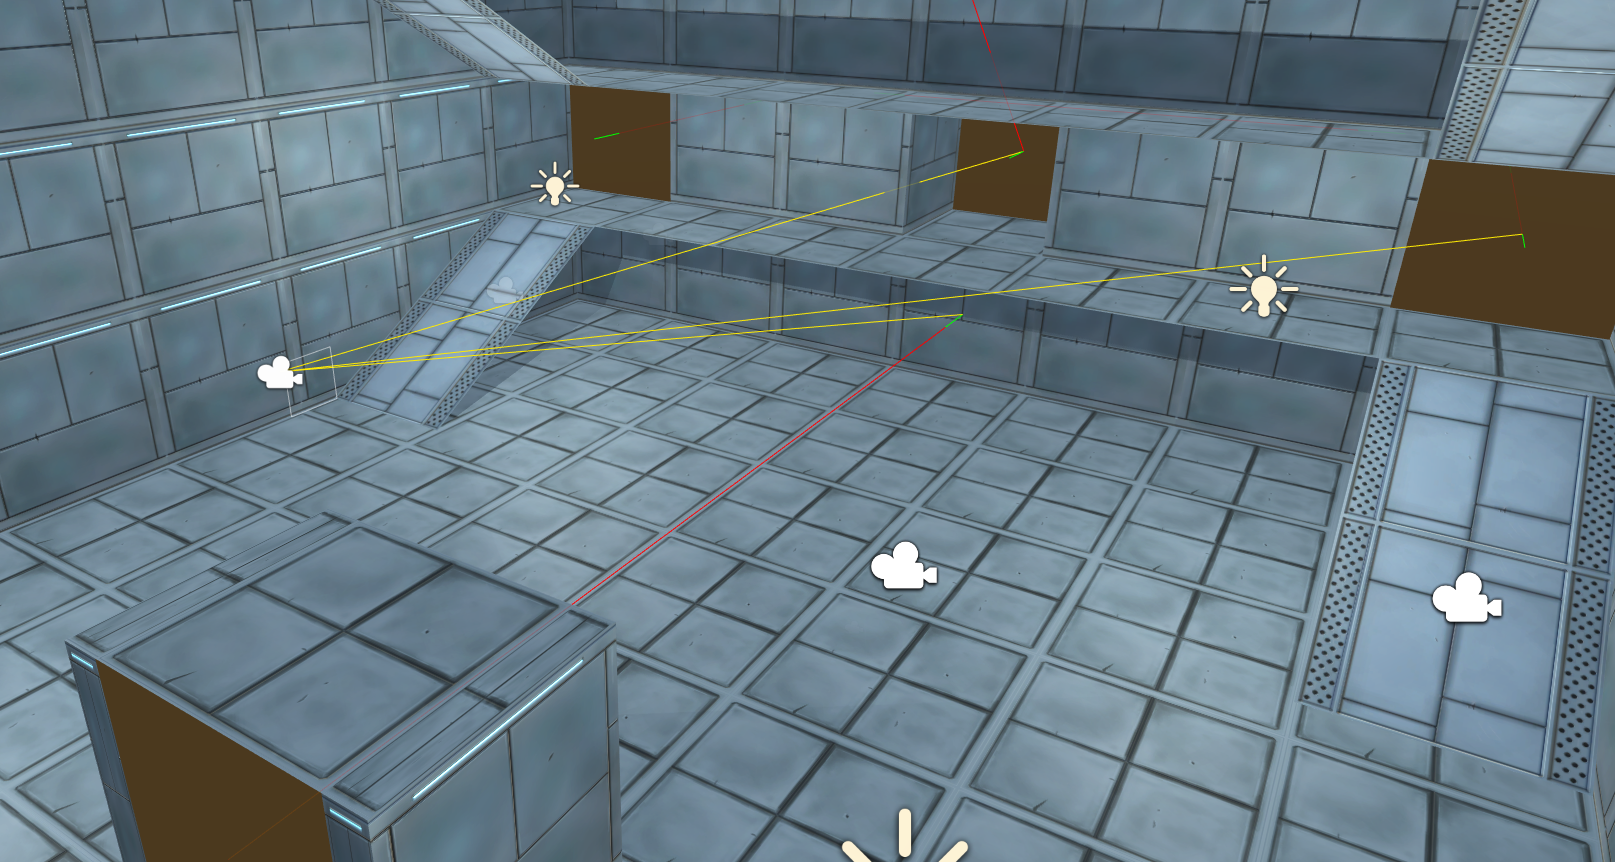
\includegraphics[width=1\textwidth]{Images/Lines_Everywhere}
			\centering
			\caption{Test scene using textured objects}
			\label{design:fig:design:tex}
		\end{figure}

		\subsubsection{Non-Euclidean Scene}

			The non-Euclidean test scene (as seen in \autoref{design:fig:design:ne}) was the first of the two scenes to be designed for the experiments.
			As a way to ensure the participants could experience a variety of the possibilities of non-Euclidean environments, a mixture of effects were chosen to be included in the scene, as labelled in \autoref{design:fig:design:ne} by the letters and corresponding red lines.

			\begin{figure}[h]
				\includegraphics[width=1\textwidth]{Images/NE_Layout}
				\centering
				\caption{Labelled layout of the Non-Euclidean experiment scene}
				\label{design:fig:design:ne}
			\end{figure}

			Point \enquote{A} represents the connection shown in \autoref{design:fig:game}, which is an example of an area appearing to contain a larger area than expected from its surroundings.
			Connection \enquote{B} represents what appears to be a direct corridor to a user which both takes a shorter path than would be expected by the two parallel paths, but also appears to occupy the same space as another corridor which runs perpendicular to it.
			Connection \enquote{C} appears to a user that they are able to walk directly between two completely separate areas of the room, both of which are on different levels (Note the corridor to the right of the \enquote{C} marker is a ramp leading down towards \enquote{D}).
			Finally, connection \enquote{D} gives the impression that the user is walking around a seemingly endless series of turns, however when the user turns back from where they came from, they find they have not travelled anywhere.

			The ramp connecting the two levels in the scene (As seen between points \enquote{C} and \enquote{D} in \autoref{design:fig:design:ne}) is at an angle of 20\degree, below the 21.98\degree critical angle for perceiving affordance when in VR \cite{Regia-Corte2012}.

		\subsubsection{Standard Scene}
			The standard Euclidean scene (as seen in \autoref{design:fig:design:standard}) was designed to follow a similar layout to the non-Euclidean one, or as close as could be possible with the geometric constraints.
			This decision was made to attempt to limit the factors that could affect the participant's immersion within the scenes, as a way to ensure that the results from the experiments are as consistent as possible.

			\begin{figure}[H]
				\includegraphics[width=0.7\textwidth]{Images/Standard_Layout}
				\centering
				\caption{Layout of the standard Euclidean experiment scene}
				\label{design:fig:design:standard}
			\end{figure}


	% Experiment
	\chapter{Experiment}
\label{exp}
\begin{multicols*}{2}

	\section{Introduction}
	Here I will give a brief overview of the experiments that I will have conducted, the variations that they have between them, and why I chose those variations.

	\section{Experiments}
		\subsection{Control - Standard Euclidean Geometry}
		Here I will talk about the results from the control experiment, which will give a good baseline as to the level of immersion a user would have in the system when subject to standard Euclidean geometry.

		\subsection{Mix - Euclidean $\rightarrow$ Non-Euclidean}
		Here I will talk about results specific to the experiment where the user starts off in a standard Euclidean world, but where the world switches to non-Euclidean spaces towards the end of their path.

		\subsection{Mix - Non-Euclidean $\rightarrow$ Euclidean}
		Here I will talk about results specific to the experiment where the user starts off in a non-Euclidean world, but switches to use regular Euclidean space towards the end of their path.

		\subsection{Non-Euclidean}
		Here I will talk about the results from the experiment where the user will be subject to non-Euclidean space for the duration of the experiment.

	\section{Summary}
	Here I will be evaluating the results of the experiments, covering any trends that appeared between the various experiments, discussing potential impacts from the results, as well as covering any additional notes that were provided about the experiments from the participants which weren't directly related to the specific experiment they were part of.

\end{multicols*}

	\begin{figure}
		\label{exp:fig:standard_immersion}
		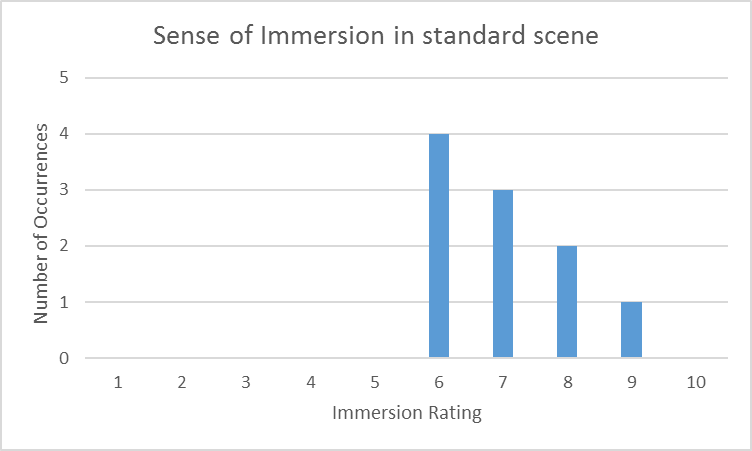
\includegraphics[width=0.7\textwidth]{Images/Standard_Immersion}
		\centering
		\caption{Immersion rating in standard geometry test scene}
	\end{figure}

	\begin{figure}
		\label{exp:fig:standard_comfort}
		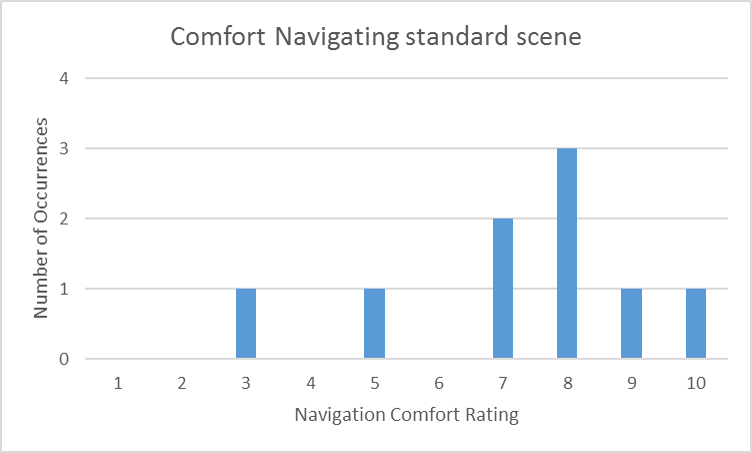
\includegraphics[width=0.7\textwidth]{Images/Standard_Comfort}
		\centering
		\caption{Navigation Comfort rating in standard geometry test scene}
	\end{figure}

	\begin{figure}
		\label{exp:fig:standard_relation}
		\includegraphics[width=0.7\textwidth]{Images/Standard_Relation}
		\centering
		\caption{Relation between sense of immersion and navigation comfort in standard geometry test scene}
	\end{figure}

	\begin{figure}
		\label{exp:fig:ne_immersion}
		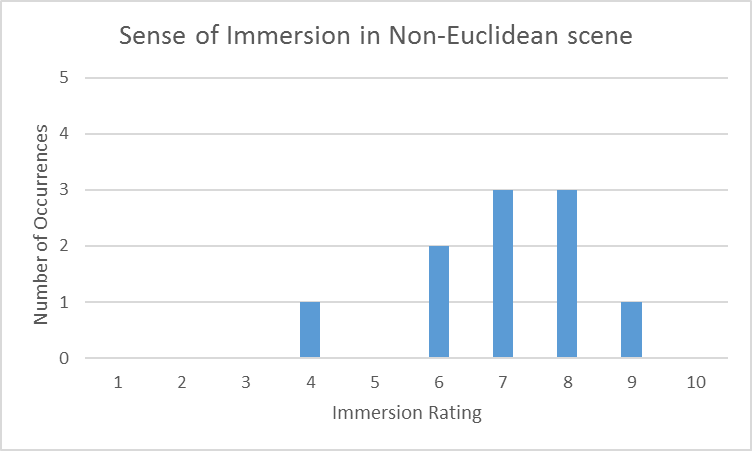
\includegraphics[width=0.7\textwidth]{Images/NE_Immersion}
		\centering
		\caption{Immersion rating in Non-Euclidean geometry test scene}
	\end{figure}

	\begin{figure}
		\label{exp:fig:ne_comfort}
		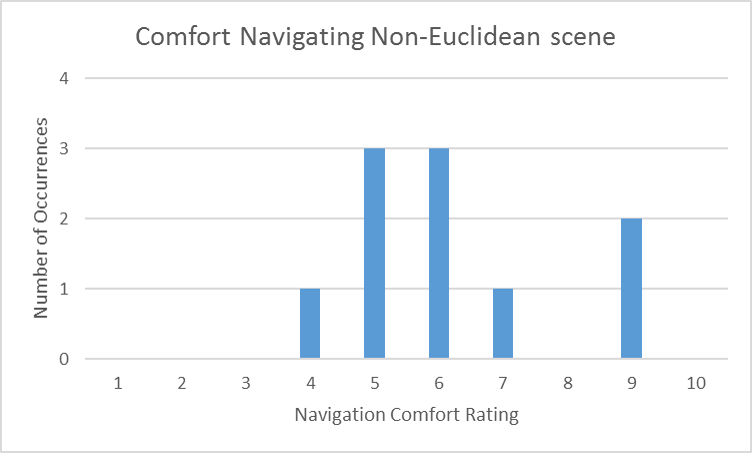
\includegraphics[width=0.7\textwidth]{Images/NE_Comfort}
		\centering
		\caption{Navigation Comfort rating in Non-Euclidean geometry test scene}
	\end{figure}

	\begin{figure}
		\label{exp:fig:ne_relation}
		\includegraphics[width=0.7\textwidth]{Images/NE_Relation}
		\centering
		\caption{Relation between sense of immersion and navigation comfort in Non-Euclidean geometry test scene}
	\end{figure}

	\begin{figure}
		\label{exp:fig:compare_immersion_exp1}
		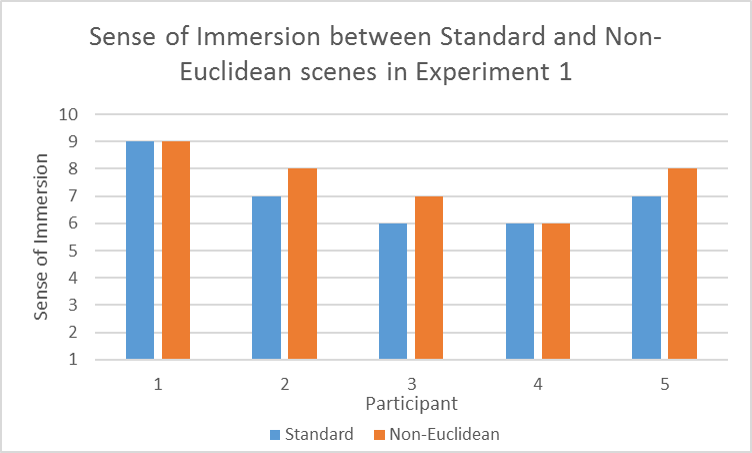
\includegraphics[width=0.7\textwidth]{Images/Compare_Immersion_Exp_1}
		\centering
		\caption{Comparison of participants sense of immersion in the two test scenes, from Experiment 1}
	\end{figure}

	\begin{figure}
		\label{exp:fig:compare_immersion_exp2}
		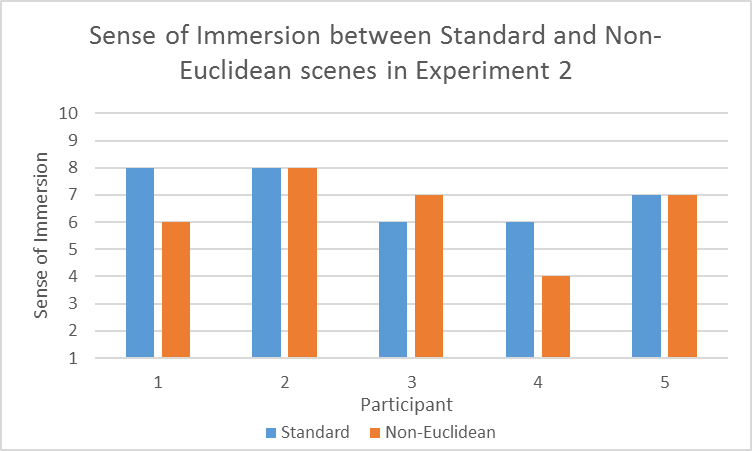
\includegraphics[width=0.7\textwidth]{Images/Compare_Immersion_Exp_2}
		\centering
		\caption{Comparison of participants sense of immersion in the two test scenes, from Experiment 2}
	\end{figure}

	\begin{figure}
		\label{exp:fig:compare_immersion_variation}
		\includegraphics[width=0.7\textwidth]{Images/Compare_Immersion_Variation}
		\centering
		\caption{Mean values, and variation of Range for Immersion in the two test scenes}
	\end{figure}

\begin{multicols*}{2}

\end{multicols*}
	
	% Project Evaluation
	\chapter{Project Evaluation}
\label{eval}
\begin{multicols*}{2}

	% This is the one bit where you can talk in the first person, so go wild.

\end{multicols*}

	% Conclusion
	\chapter{Conclusion}
\label{conclusion}
\begin{multicols*}{2}

	Here is where I will conclude the report as a whole, covering the results of the experiment, how they match up to the information learned from the existing literature review, as well as any further work which could be done on the subject area.

\end{multicols*}

	% Bibliography
	\nocite{*}	% Make all entries in the bibliography file appear in the references section, even if not cited directly
	\begingroup
		\chapter{References}
		\label{ref}

		\renewcommand{\chapter}[2]{}		% Change chapter behaviour to make it not force the bibliography onto the following page
		\bibliographystyle{apalike}			% Set the bibliography to use APA formatting
		\bibliography{FinalYearProject}	    % Select the file to use for the bibliography
	\endgroup

	% Appendices
	\chapter{Appendix}
\label{appendix}

	% List of Figures
	\begingroup
		\section{List of Figures}
		\label{appendix:figures}

		Below are a list of the figures which are present in the document, along with their corresponding page number.

		\renewcommand{\chapter}[2]{}		% Change chapter behaviour to make it not force the list of figures onto the following page
		\listoffigures						% Display the list of figures
	\endgroup

	\section{Code Samples}
	\label{appendix:code}

		Below are code snippets for sections or complete functions that have specifically been referenced in the body of the report.

		\begin{lstlisting}[caption="Camera Positioning - CameraRenderPosition.cs", label=appendix:code:camera]
Vector3 offset = PointOfView.position - _player.position + ((_player.position - _player.parent.parent.position) / 2);

// Position and rotate the cameras depending on the type of illusion they are going for
if (!Inverse) {
	Moveable.position = Helper.RotatePointAroundPivot(RenderPosition.position - offset, RenderPosition.position, _relativePortalRot.eulerAngles);
	Moveable.rotation = _relativePortalRot * Quaternion.Euler(rotationOffset + _defaultRot - _normalisedDefaultRot);
} else {
	Moveable.position = RenderPosition.position - offset;
	Moveable.rotation = _relativePortalRot * Quaternion.Euler((RenderPosition.transform.up == Vector3.up ? rotationOffset : -rotationOffset) + _defaultRot - _normalisedDefaultRot + new Vector3(0, 180f, 0));
}

// Set the near clipping plane of the camera to only render starting from the closest visible area
_cam.nearClipPlane = (Helper.FindClosestPoint(_bounds, transform.position) - transform.position).magnitude / 2f;
		\end{lstlisting}

		\begin{lstlisting}[caption="Player Positioning - CameraRenderPosition.cs", label=appendix:code:player]
/// <summary>
/// Re-Position the player from their current position to the equivelant position of its point of view, depending on their relative position
/// </summary>
/// <param name="player">Player to potentially transport</param>
/// <param name="centre">Centre of the currently colliding object</param>
/// <param name="forward">Forward vector of the currently colliding object</param>
public void positionPlayer (Collider player, Vector3 centre, Vector3 forward) {
	// Get the distance vector between the player and the centre of the currently colliding object
	Vector3 distance = player.transform.position - centre;
	Quaternion inverseFlip = Quaternion.Euler(0, 0, 0);

	// If only one of the points are inverted, make sure to flip the player
	if (Inverse != _linkedScript.Inverse) {
		inverseFlip = Quaternion.Euler(0, 180f, 0);
	}

	// If the player is more than half way through the object, transport them to the linked area
	if (Vector3.Dot(distance.normalized, forward) < 0) {
		// Set player position
		distance = Helper.RotatePointAroundPivot(distance, Vector3.zero, (_relativePlayerRot.eulerAngles + inverseFlip.eulerAngles));
		player.transform.position = PointOfView.position;
		player.transform.position += distance;

		// Set player rotation
		rotationOffset += _relativePlayerRot.eulerAngles + inverseFlip.eulerAngles;
		player.transform.rotation = _relativePlayerRot * inverseFlip * player.transform.rotation;

		// Update the players momentum
		_playerControl.UpdateMoveThrottle(_relativePlayerRot * inverseFlip * _playerControl.GetMoveThrottle());
	}
}
		\end{lstlisting}

	\section{Ethics Review}
	\label{appendix:ethics}
		A completed and signed copy of the Project Ethical Review Form can be found on the following two pages.

		\includepdf[pages={-},scale=0.9]{"Resources/Ethical Review Scan"}

	\section{Questionnaire}
	\label{appendix:question}
		A blank copy of the form used to gather the feedback discussed in Chapter \ref{exp} can be seen in the following two pages. The completed versions of the forms containing the raw data gathered are available upon request. Either the 1 or 2 were highlighted under the 'Experiment' section at the top of each page before being given to a participant, as a reference to which experiment the form was for, without indicating to the participant the nature of the experiment.

		\includepdf[pages={-},scale=1]{"Resources/Project Feedback Questionnaire"}
		

% End the document
\end{document}
